\section{\textcolor{blue}{Thiết kế kiến trúc}} % Requirement elicitation

\subsection{Kiến trúc MVC}
$\indent$ Nhóm tác giả lựa chọn một trong những kiến trúc rất phổ biến đó là MVC (Model - View - Controller) để thiết kế hệ thống HCMUT\_SPSS.
\begin{figure}[H]
    \begin{center}
    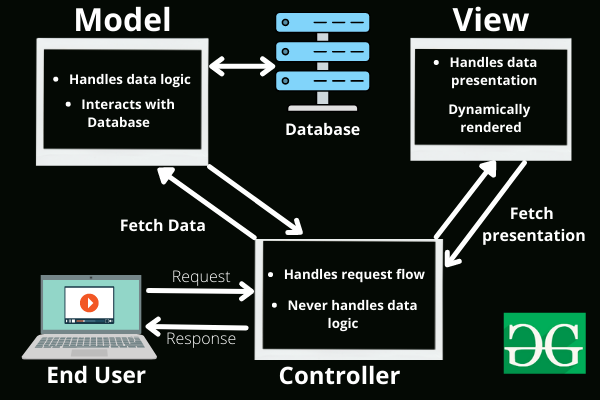
\includegraphics[width=0.9\textwidth]{Images/Box-line + Deployment/MVC.png}
        \caption{Mô hình kiến trúc MVC \textcolor{blue}{(tham khảo từ GeeksforGeeks.org}}
    \end{center}
\end{figure}
$\indent$ \textbf{Ưu điểm của MVC:}
\begin{itemize}
    \item Tách biệt giữa các thành phần: Mô hình MVC tách biệt các thành phần của ứng dụng thành Model, View và Controller. Điều này giúp làm rõ trách nhiệm của từng thành phần, dễ quản lý và duy trì mã nguồn.
    \item Dễ bảo trì: Việc tách biệt các thành phần cho phép bạn dễ dàng thay đổi hoặc cải tiến một phần của ứng dụng mà không cần sửa đổi toàn bộ mã nguồn.
    \item Phát triển đồng bộ: Mô hình MVC cho phép nhiều lập trình viên làm việc cùng một lúc trên các phần khác nhau của ứng dụng mà không gây xung đột về mã nguồn.
    \item Tích hợp dễ dàng: Có thể thay đổi hoặc thay thế một phần của ứng dụng mà không cần ảnh hưởng đến các phần khác, giúp tích hợp các thành phần mới một cách dễ dàng.
    \item Dễ kiểm thử: Mô hình MVC dễ kiểm thử vì bạn có thể kiểm tra riêng lẻ các thành phần Model, View và Controller mà không cần chạy toàn bộ ứng dụng.
\end{itemize}
$\indent$ \textbf{Nhược điểm của MVC:}
\begin{itemize}
    \item Độ trễ cao: Sử dụng mô hình MVC có thể tạo ra một chút độ trễ do việc truyền thông qua các thành phần khác nhau.
    \item Khó quản lý khi ứng dụng phức tạp: Đối với các ứng dụng rất phức tạp, quản lý các thành phần và tương tác giữa chúng có thể trở nên khó khăn.
\end{itemize}
$\indent$Từ việc tìm hiểu và phân tích những ưu nhược điểm của kiến trúc MVC. Nhóm tác giả quyết định lựa chọn kiến trúc này bởi vì:
\begin{itemize}
    \item Vì MVC tách biệt giữa các thành phần nên việc phân công giữa các thành viên sẽ dễ dàng hơn. Hơn nữa việc tích hợp và phát triển đồng bộ sẽ phù hợp cho dự án gồm nhiều thành viên.
    \item SPSS là một hệ thống vừa và nhỏ do đó sẽ giảm bớt khó khăn trong việc quản lý ứng dụng.
    \item Hơn hết, MVC là một mô hình phổ biến và được áp dụng rộng rãi. Vì thế việc sử dụng mô hình này như một cơ hội để nhóm tác giả tìm hiểu và vận dụng một cách hiệu quả sau này.
\end{itemize}
\subsection{Architectural diagram và Deployment diagram}
\subsubsection{Architectural diagram cho toàn hệ thống}
\begin{figure}[H]
    \begin{center}
    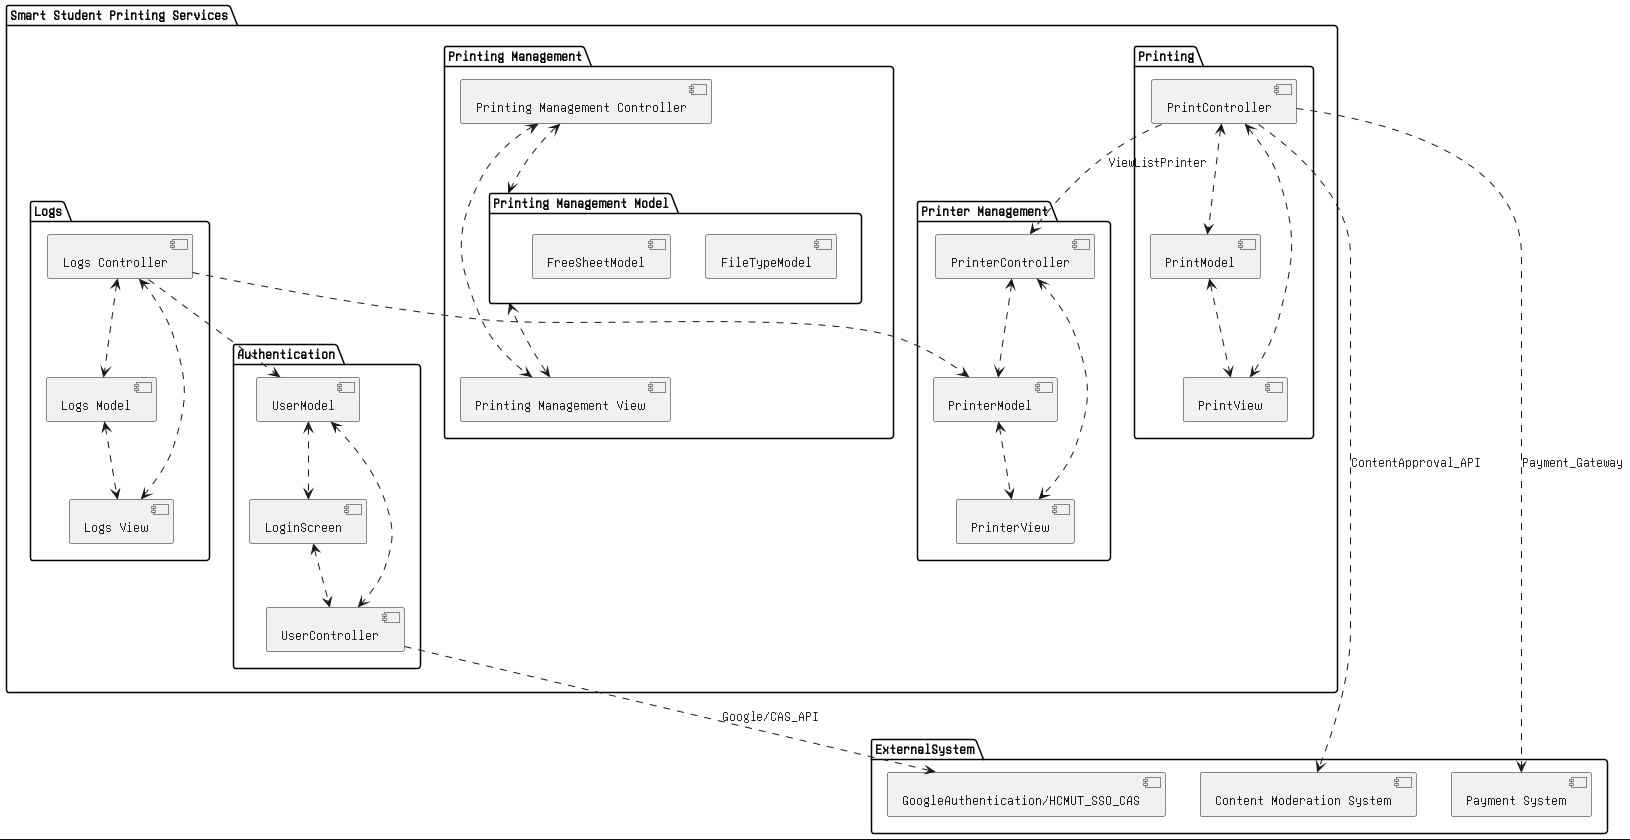
\includegraphics[width=1\textwidth]{Images/Box-line + Deployment/ArchitectureDiagram.drawio.png}
\caption{Architectural diagram}
    \end{center}
\end{figure}
Để xem rõ hơn bản vẽ của nhóm, truy cập tại \href{https://drive.google.com/file/d/1vgr0dHbZ-yCTvMx9BN5ZEvlmdY8I_FYY/view?usp=sharing}{đây} 
\begin{itemize}
    \item \textbf{Authentication:}
    \begin{itemize}
        \item \textbf{UserModel:} Quản lý thuộc tính và logic của User để xác thực tài khoản.
        \item \textbf{LoginScreen:} Phần giao diện người dùng liên quan đến xác thực.
        \item \textbf{UserController:} Điều khiển logic và tương tác với UserModel và LoginScreen. Kết nối với Google/HCMUT\_SSO.
    \end{itemize}
    \item \textbf{Printing:}
    \begin{itemize}
        \item \textbf{PrintModel:} Quản lý thuộc tính in ấn và tài liệu.
        \item \textbf{PrintView:} Giao diện người dùng cho việc in tài liệu.
        \item \textbf{PrintController:} Điều khiển logic in ấn và sự tương tác giữa PrintModel và PrintView
    \end{itemize}
    \item \textbf{Printer Management:}
    \begin{itemize}
        \item \textbf{PrinterModel:} Quản lý các thuộc tính và xử lý logic dữ liệu liên quan tới máy in
        \item \textbf{PrinterView:} Giao diện người dùng cho quản lý máy in.
        \item \textbf{PrinterController:} Điều khiển logic quản lý máy in, tương tác với PrinterModel và PrinterView.
    \end{itemize}
    \item \textbf{Printing Management:}
    \begin{itemize}
        \item \textbf{Printing Management Model:} Quản lý thông tin quản lý in ấn. Gồm 2 model đó à FreeSheetModel (quản lý thông tin về số giấy, ngày tặng miễn phí cho user) và FileTypeModel (quản lý dữ liệu về các loại file được phép in).
        \item \textbf{Printing Management View:} Giao diện người dùng cho quản lý in ấn.
        \item \textbf{Printing Management Controller:} Điều khiển logic quản lý in ấn, tương tác với Printing Management Model và Printing Management View.
    \end{itemize}
    \item \textbf{Logs:}
    \begin{itemize}
        \item \textbf{LogsModel:} Quản lý và lưu trữ lịch sử in ấn.
        \item \textbf{LogsView:} Giao diện người dùng cho xem lịch sử in ấn.
        \item \textbf{LogsController:} Điều khiển logic xem lịch sử in ấn, tương tác với Logs Model và Logs View. Ngoài ra còn tương tác với UserModel và PrinterModel để yêu cầu một số thông tin như ID user, ID máy in
    \end{itemize}
\end{itemize}
\subsubsection{Deployment diagram cho toàn hệ thống}
\subsubsubsection{Bản vẽ Deployment Diagram}
\begin{figure}[H]
    \begin{center}
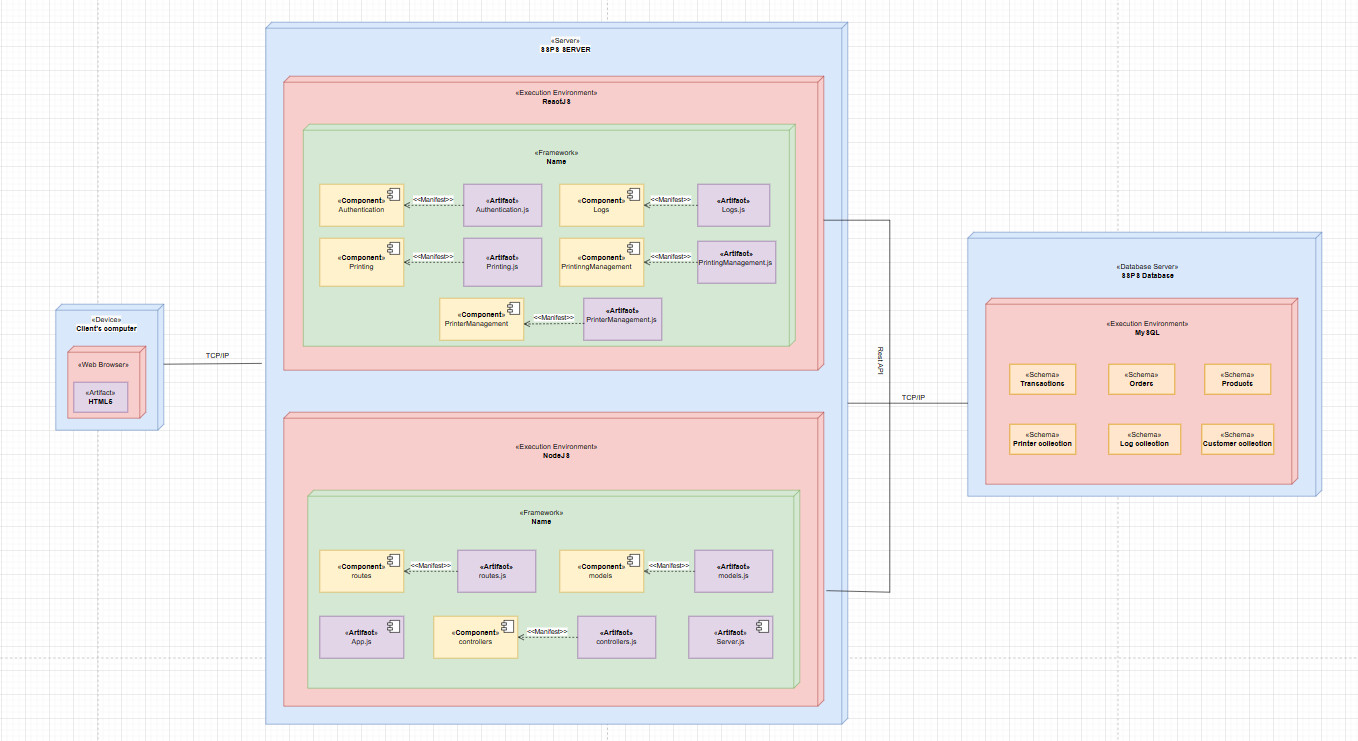
\includegraphics[width=0.9\textwidth]{Images/Box-line + Deployment/deployment.jpg}
        \caption{Deployment diagram}
    \end{center}
\end{figure}
Để xem rõ hơn bản vẽ của nhóm, truy cập tại \href{https://drive.google.com/file/d/1t1EVsOUQxixdM85v2Ch99MjhRM3ihQc9/view?usp=sharing}{đây} .
\subsubsubsection{Mô tả Deployment Diagram}
\begin{itemize}
    \item Hệ thống là một ứng dụng Web, được phát triển theo kiến trúc MVC, bao gồm 3 máy chủ chính: Client, Server và Database Server.
    \item Máy chủ Client sẽ kết nối với Server thông qua giao thức TCP/IP, dữ liệu nhận được từ
Server là các file hiện thực giao diện và sẽ được hiển thị trên browser website tại máy
tính người dùng (Client) thông qua trình đọc HTML5 được nhúng trong trình duyệt.
    \item Máy chủ Server bao gồm môi trường thực thi (execution environment) các module chức
năng chính của hệ thống. Môi trường thực thi phía \textbf{back-end} là \textbf{NodeJS}, sử dụng Framework là \textbf{Express.js}, bao gồm 5 component chính là:
    \begin{itemize}
        \item \textbf{Authentication}: Chứa mã nguồn cho module xác thực người dùng.
        \item \textbf{Printing}: Chứa mã nguồn cho module in ấn.
        \item \textbf{PrinterManagement}: Chứa mã nguồn cho module quản lý máy in.
        \item \textbf{PrintingManagement}: Chứa mã nguồn cho module quản lý in ấn.
        \item \textbf{Logs}: Chứa mã nguồn cho module xem lịch sử in ấn.

    \end{itemize}
Môi trường thực thi phía \textbf{front-end} là \textbf{ReactJS}, sử
dụng Framework là \textbf{Material UI}, bao gồm 5 component chính là:
\begin{itemize}
    \item \textbf{Routes}: Chứa các tệp định tuyến cho từng module.
    \item \textbf{Controllers}: Chứa các tệp điều khiển cho từng module để xử lý logic kinh doanh.
    \item \textbf{Models}: Chứa các tệp mô hình dữ liệu (ORM) cho cơ sở dữ liệu.
    \item \textbf{App.js}: Cấu hình ứng dụng Express và gắn các tệp định tuyến.
    \item \textbf{Server.js}: Khởi động máy chủ Node.js.
\end{itemize}
    \item Máy chủ Server sẽ kết nối với Database Server thông qua giao thức TCP/IP, để truy
xuất dữ liệu hiển thị lên giao diện hoặc cập nhật lại dữ liệu mỗi khi người dùng tương
tác với ứng dụng, sau đó dữ liệu sau khi cập nhật sẽ được truyền qua giao thức TCP/IP
sang Server và truyền sang máy Client để cập nhật lại giao diện.
    \item Máy chủ Database bao gồm môi trường thực thi là DBMS MySQL.Máy chủ Database lưu trữ các thông tin bao gồm: \textbf{Log collection}, \textbf{Customer collection}, \textbf{Printer collection}, \textbf{Transactions}, \textbf{Orders}, \textbf{Products} ở dạng bảng có cấu trúc và các mối quan
hệ với nhau.
\end{itemize}
\subsection{Component diagram}
\subsubsection{Xác thực}
\begin{figure}[H]
    \begin{center}
        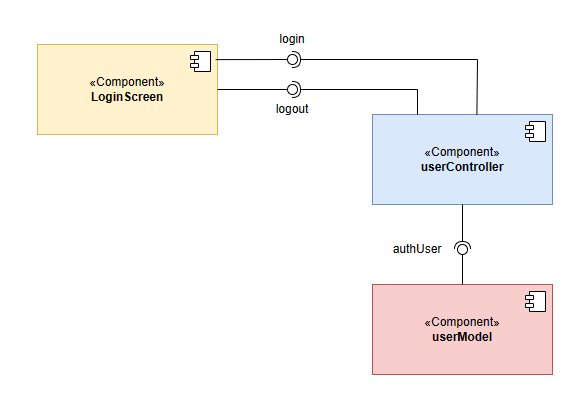
\includegraphics[width=0.9\textwidth]{Images/Architecture Design/Authen_Component.png}
        \caption{Component diagram cho module xác thực}
    \end{center}
\end{figure}
\textbf{Mô tả:}\par
Trong component diagram của module xác thực, tầng view gồm có 1 component đó là LoginSrceen với chức năng là cung cấp giao diện cho người dùng đăng nhập tài khoản. Tầng controller gồm có 1 component đó là userController với chức năng là cung cấp các phương thức để xác thực tài khoản. Tầng model gồm có 1 component đó là userModel với chức năng chính là lưu trữ và thực hiện truy vấn dữ liệu liên quan tới tài khoản người dùng (xác thực tài khoản).

\subsubsection{In}
\begin{figure}[H]
    \begin{center}
        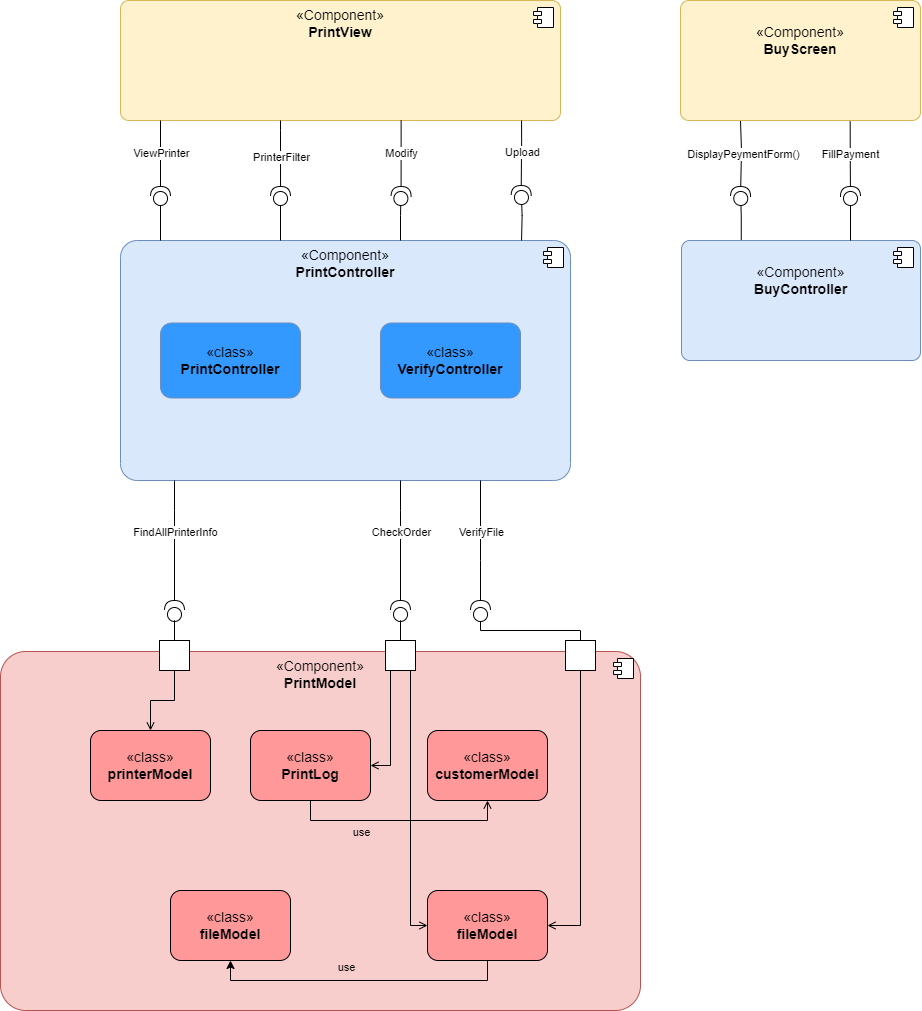
\includegraphics[width=0.9\textwidth]{Images/Architecture Design/Printing_Component.png}
        \caption{Component diagram cho module in}
    \end{center}
\end{figure}
\textbf{Mô tả:}\par
Trong component diagram của module in, tầng view gồm có 2 component là \textbf{PrintView} với chức năng cung cấp giao diện cho người dùng thực hiện các thao tác (Chọn máy in, chuyển sang mua giấy) và \textbf{BuyScreen} với chức năng cung cấp giao diện cho người dùng thực hiện mua giấy. Tầng controller gồm có 2 component là \textbf{PrintController} bao gồm 2 class là \textbf{PrintController} và \textbf{VerifyController} với chức năng cung cấp các phương thức tìm kiếm thông tin và chọn máy in, component \textbf{BuyController} với chức năng cung cấp các phương thức tạo form mua giấy. Tầng model gồm có 1 component là PrintModel với chức năng chính là lưu trữ và thực hiện truy vấn dữ liệu liên quan đến việc in ấn (lấy thông tin máy in, kiểm tra và lưu trữ thông tin in ấn).\par

\subsubsection{Quản lý máy in}
\begin{figure}[H]
    \begin{center}
        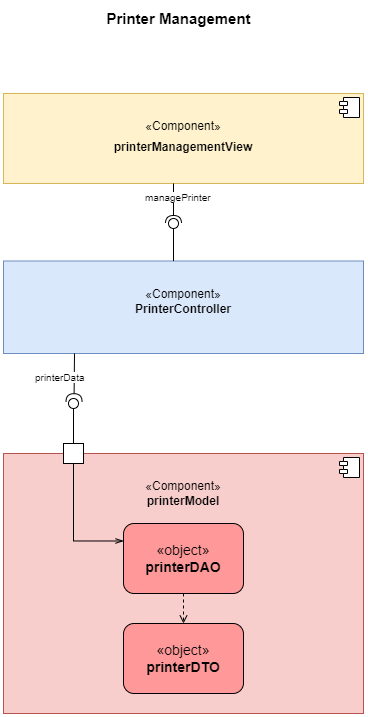
\includegraphics[width=0.4\textwidth]{Images/Architecture Design/PM_Component.png}
        \caption{Component diagram cho module quản lý máy in}
        \label{fig:arch}
    \end{center}
\end{figure}
\textbf{Mô tả:}\par
Trong component diagram của module quản lý máy in, tầng view gồm có 1 component đó là printerManagementView với chức năng là cung cấp giao diện cho SPSO quản lý máy in (thêm, xóa, kích hoạt và vô hiệu hóa máy in, xem). Tầng controller gồm có 1 component đó là printerController với chức năng là cung cấp các phương thức quản lý máy in đó là thêm, xóa, kích hoạt, vô hiệu hóa và xem. Tầng model gồm có 1 component đó là printerModel với chức năng chính là lưu trữ và thực hiện truy vấn dữ liệu liên quan đến máy in (thêm, xóa, kích hoạt, vô hiệu hóa, xem). Trong component printerModel thì sẽ có 2 object là printerDAO (giúp truy vấn đến cơ sở dữ liệu) và printerDTO (lưu trữ dữ liệu của máy in).\par
Các interface: 
\begin{itemize}
    \item managePrinter:cung cấp các phương thức giúp quản lý máy in (thêm, xóa, kích hoạt, vô hiệu hóa, xem).
    \item printerData: cung cấp API lấy dữ liệu máy in để quản lý (thêm, xóa, kích hoạt, vô hiệu hóa, xóa).
    
\end{itemize}



\subsubsection{Sửa danh mục định dạng tệp cho phép \& Quản lý tặng giấy miễn phí}

\begin{figure}[H]
    \begin{center}        
    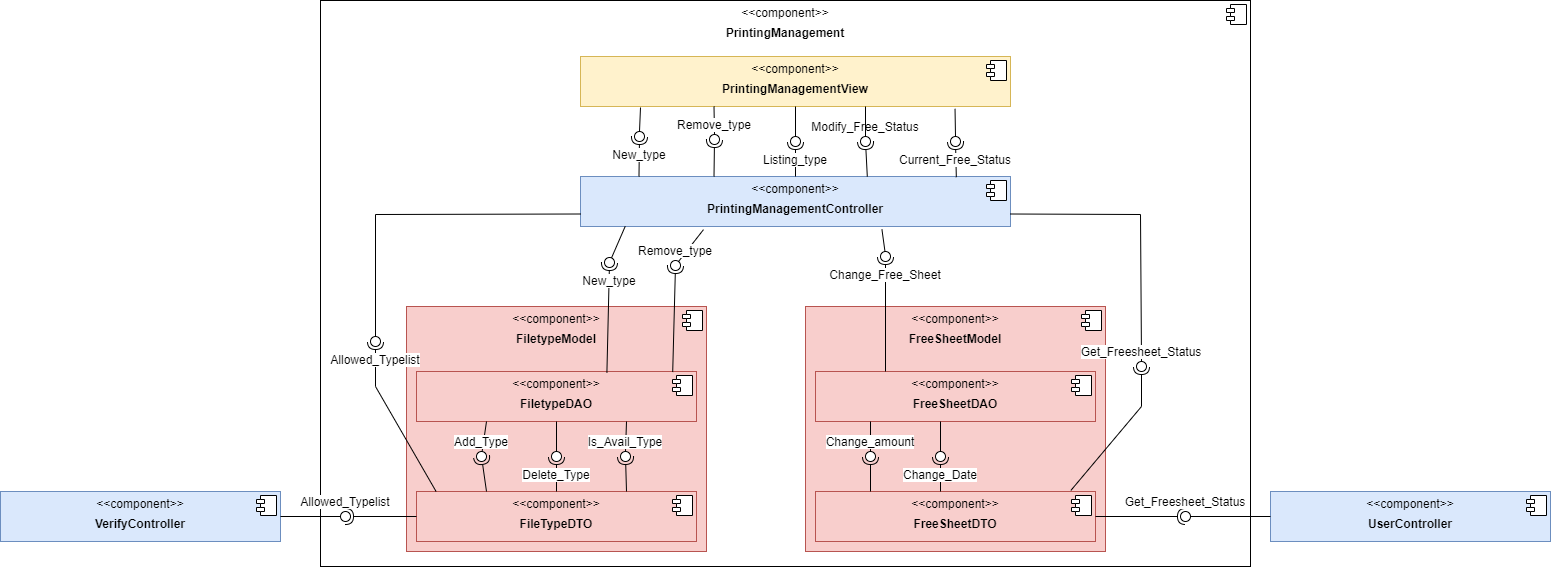
\includegraphics[width=0.8\textwidth]{Images/Architecture Design/PS_Component.png}
        \caption{Component diagram cho module quản lý định dạng}
        \label{fig:arch}
    \end{center}
\end{figure}

\textbf{Mô tả:}\par
Thành phần PrintingManagementView chứa các giao diện cần thiết cho người dùng để thực hiện yêu cầu thêm/bớt kiểu tệp được cho phép in (New\_type), (Remove\_type), xem danh sách các kiểu tệp được phép in (Listing\_type) và xem hoặc chỉnh sửa ngày tháng tặng giấy miễn phí tới thành phần PrintingManagementController. \\
Thành phần PrintingManagementController chứa các bộ xử lý những truy vấn đầu vào từ View, sau đó truyền những yêu cầu tiếp theo tương ứng tới lớp FileTypeModel hoặc FreeSheetModel. \\
Thành phần Model nhận các yêu cầu từ Controller và thực hiện nhiệm vụ như truy xuất, thay đổi cơ sở dữ liệu về danh sách kiểu tệp cho phép in hay ngày tháng tặng giấy.

\subsubsection{Lịch sử in}
\begin{figure}[H]
    \begin{center}        
    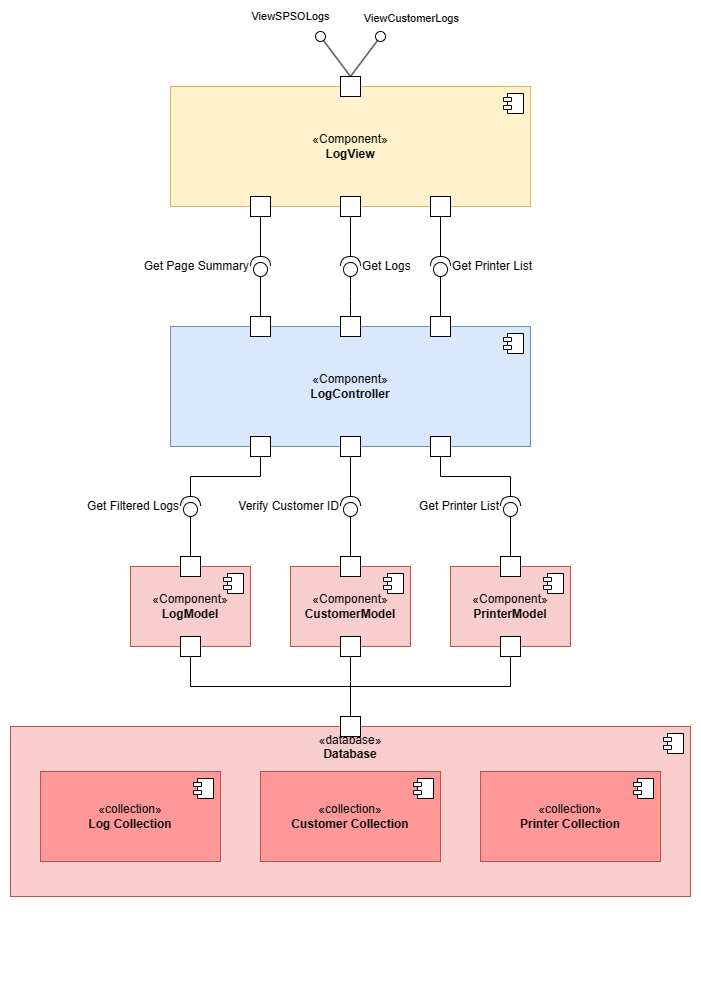
\includegraphics[width=0.8\textwidth]{Images/Architecture Design/Logging_Component.png}
        \caption{Component diagram cho module lịch sử in}
        \label{fig:arch}
    \end{center}
\end{figure}

\textbf{Mô tả:}\par
Lớp View bao gồm một thành phần LogView, cung cấp hai giao diện ViewSPSOLogs và ViewCustomerLogs để truy xuất dữ liệu lịch sử in ấn của SPSO và khách hàng. Lớp Controller có thành phần LogController, cung cấp giao diện cho LogView, bao gồm việc lấy dữ liệu lịch sử in, tóm tắt số trang và lấy danh sách máy in đang hoạt động. Lớp Model bao gồm các thành phần LogModel, CustomerModel và PrinterModel. LogController sử dụng PrinterModel để lấy danh sách máy in, sử dụng CustomerModel để kiểm tra ID khách hàng được nhập vào bộ lọc và sử dụng LogModel để lấy dữ liệu lịch sử in ấn từ cơ sở dữ liệu.\par



